% GENERATED by mb5.paper_numbers from paper/figures/figures.tex (mb5.figures)
\begin{figure*}[t]
  \centering
  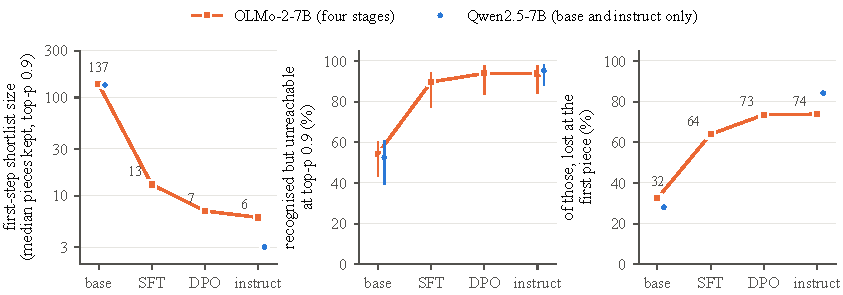
\includegraphics[width=\textwidth]{figures/fig3_stages.pdf}
  \caption{Where unreachability comes from: OLMo-2-7B after each post-training stage (pilot, 11 categories; SFT: supervised fine-tuning; DPO: preference tuning), with the Qwen2.5-7B base and instruct pair for comparison. SFT alone shrinks the first-step shortlist from 137 to 13 pieces. From base to instruct, the share of recognised entities that are unreachable at top-p 0.9 rises from 54.4\% to 93.8\%, and the share of those lost at the first piece from 32\% to 74\%. Bars: 95\% cluster-bootstrap intervals.}
  \label{fig:stages}
\end{figure*}
